\documentclass[aspectratio=169]{beamer}
\mode<presentation>
%\usetheme{Warsaw}
%\usetheme{Goettingen}
\usetheme{Hannover}
%\useoutertheme{default}

%\useoutertheme{infolines}
\useoutertheme{sidebar}
\usecolortheme{dolphin}


\setbeamersize{sidebar width left=0pt} % to remove the sidebar
\beamertemplatenavigationsymbolsempty % To remove the navigation symbols on the bottom right.
\setbeamersize{text margin left=10mm,text margin right=10mm} % Specify margins

\usepackage{amsmath}
\usepackage{amssymb}
\usepackage{listings}
\usepackage{enumerate}
\usepackage{hyperref}
\hypersetup{
    colorlinks=true,
    linkcolor=blue,
    filecolor=magenta,      
    urlcolor=cyan,
}
 
\urlstyle{same}

%some bold math symbosl
\newcommand{\Cov}{\mathrm{Cov}}
\newcommand{\Var}{\mathrm{Var}}
\newcommand{\brho}{\boldsymbol{\rho}}
\newcommand{\bSigma}{\boldsymbol{\Sigma}}
\newcommand{\btheta}{\boldsymbol{\theta}}
\newcommand{\bbeta}{\boldsymbol{\beta}}
\newcommand{\bmu}{\boldsymbol{\mu}}
\newcommand{\bW}{\mathbf{W}}
\newcommand{\one}{\mathbf{1}}
\newcommand{\bH}{\mathbf{H}}
\newcommand{\by}{\mathbf{y}}
\newcommand{\bolde}{\mathbf{e}}
\newcommand{\bx}{\mathbf{x}}

\newcommand{\cpp}[1]{\texttt{#1}}

%--------------------------------------------------
\providecommand{\abs}[1]{\lvert#1\rvert}
\providecommand{\norm}[1]{\lVert#1\rVert}
\providecommand{\Blue}[1]{\textcolor{blue}{#1}}
\providecommand{\Red}[1]{\textcolor{red}{#1}}
\newcommand{\celsius}{\ensuremath{^\circ}C}
\newcommand\thfore{\mathord{\therefore}\,}
%------------------------------------------------------------------

\title{Lecture 3. Matrix Representation of Graphs: Adjacency Matrix}
%\author{\includegraphics[width=.5\textwidth,height=.5\textheight]{lecture4-fig0.png}}

\date{ }
%------------------------------------------------------------------


\begin{document}

\frame[plain]{\titlepage}

\begin{frame}[plain]{What is a matrix?}

A \Blue{matrix} is a rectangular array of elements arranged in \Blue{horizontal rows} 
and \Blue{vertical columns}, and usually enclosed in brackets.
 
   \begin{columns}[c]
   \column{.4\textwidth} 
  
    \center  
    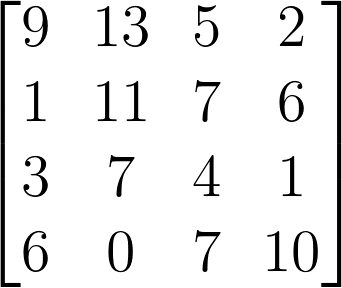
\includegraphics[height=2.2cm]{./img/lecture3-fig1.png}
    
    \medskip
    
    The above is a $4\times 4$ matrix (4 rows and 4 columns).
   
   \column{.6\textwidth} 
    
     
     \[ \mathrm{A}\ = \left[ \begin{array}{cccc}
                            a_{11} & a_{12} & \cdots & a_{1n} \\
                            a_{21} & a_{22} & \cdots & a_{2n} \\
                            \vdots &   \vdots     & \vdots & \vdots        \\
                            a_{m1} & a_{m2} & \cdots & a_{mn} 
                           \end{array}
                    \right]                    
   \]   
   \medskip
   
   \ \ \ \ \ \ \ \ \ \ \ \ \   $A$ is an $m\times n$ matrix. \\
   \ \ \ \ \ \ \ \ \ \ \ \ \ ($m$ rows and $n$ columns.)
    
    
  \end{columns}


 \end{frame}




\begin{frame}[plain]{Adjacency Matrix}

 If an \Red{unweighted simple} graph $G$ contains 
   a total of $n$ vertices, we can define an $n\times n$ matrix $A$ by
  \[ 
   a_{ij} = \left\{ \begin{array}{ll}
       1 & \mbox{if}\ [v_i, v_j] \mbox{\ is an edge of\ } G\\
       0 & \mbox{if there is no edge joining}\ v_i\ \mbox{and}\ v_j
       \end{array}
       \right.
\] 
The resulting matrix $A=[a_{ij}]$ is called the \Blue{adjacency matrix} of the graph $G$.
\medskip

\pause

{\bf Example 3.1}. Construct an adjacency matrix of the graph below.
\medskip

  We order the vertices as $a, b, c, d$. That is, $v_1 = a, v_2=b, v_3=c, v_4=d$.
  The matrix representing this graph is

 \begin{center}
  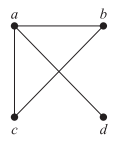
\includegraphics[height=3cm]{./img/lecture3-fig2a.png}\hspace{.4in}\pause
   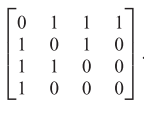
\includegraphics[height=2.7cm]{./img/lecture3-fig2b.png}
 \end{center}
 
\end{frame}

\begin{frame}[plain]{ }

For a \Red{weighted simple} graph $G$
 \[ 
   a_{ij} = \left\{ \begin{array}{ll}
       w_{ij} & \mbox{if}\ \mbox{the\ \Red{length}\ of\ the\ edge}\ [v_i, v_j]
         = w_{ij}\\
       0 & \mbox{if there is no edge joining}\ v_i\ \mbox{and}\ v_j
       \end{array}
       \right.
\]  
The resulting matrix $A=[a_{ij}]$ is called the \Blue{adjacency matrix} of the graph $G$.
\medskip

\pause

{\bf Example 3.2}. Construct an adjacency matrix of the graph below.
\medskip

 \begin{center}
  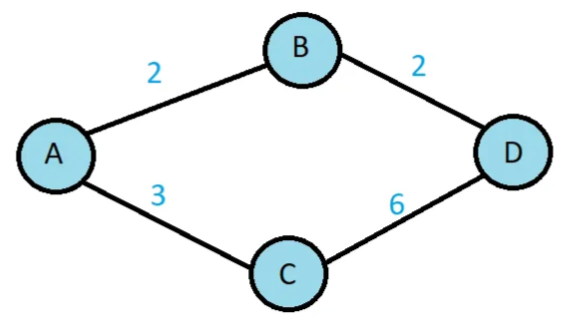
\includegraphics[height=2.2cm]{./img/lecture3-fig3.png}\hspace{.5in}\pause
   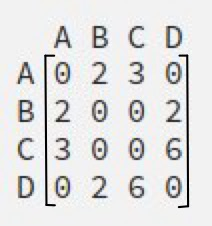
\includegraphics[height=2.7cm]{./img/lecture3-fig3b-1.jpg}
 \end{center}
 

\end{frame}


\begin{frame}[plain]{}

 {\bf Practice 3.3}. Draw an unweighted simple graph with the adjacency matrix
 
  \begin{center}
  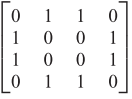
\includegraphics[height=2cm]{./img/lecture3-fig4a.png}\hspace{.4in}\pause
   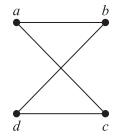
\includegraphics[height=2.4cm]{./img/lecture3-fig4b.png}
 \end{center}
 
 \pause
 
 Note that an adjacency matrix of a  graph is based on the ordering chosen for the vertices.
 Hence, there may be as many as $n!$ different adjacency matrices for a graph with $n$ vertices,
 because there are $n!$ different orderings of $n$ vertices. \medskip
 
 Also, note that adjacency matrices of undirected graphs are \Blue{symmetric}. \pause
 \medskip
 
 {\bf Question.}  What is the sum of the entries in a row of the adjacency
matrix for an undirected simple graph?
 
\end{frame}

\begin{frame}[plain]{}

Adjacency matrices can also be used to represent undirected graphs with loops and with
multiple edges. 
\begin{itemize}
  \item A \Red{loop} at the vertex $v_i$ is represented by a \Red{1}
   at the $(i, i)$th position of the adjacency matrix.~\footnote{Some books assign 
   \Red{2} for a loop. But here, we assign \Red{$1$} to indicate the number of
   edges directly associated with two adjacent vertices. } 
\item When multiple edges connecting the same pair of vertices $v_i$ and $v_j$, or multiple
loops at the same vertex, are present, 
 the $(i, j)$th entry of the adjacency matrix equals the number of edges that are associated 
to $[v_i, v_j]$.
\end{itemize}

\medskip


 {\bf Example 3.4}. Use an adjacency matrix to represent the graph
 
 \begin{center}
  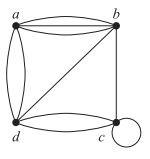
\includegraphics[height=2.8cm]{./img/lecture3-fig5a.png}\ \ \ \ \ \ \  \pause
  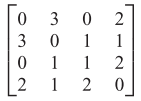
\includegraphics[height=2.2cm]{./img/lecture3-fig5b.png}
 \end{center}
 \medskip

 
\end{frame}


\begin{frame}[plain]{}

 The adjacency matrix for a \Red{directed} graph does not have to be symmetric,
 because there may not be an edge from $v_j$ to $v_i$ when there is an edge from 
 $v_i$ to $v_j$.
 \medskip
 
{\bf Practice 3.5}.  Use an adjacency matrix to represent the directed graph
 
 \begin{center}
  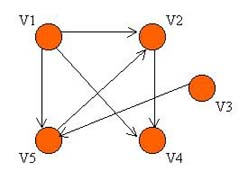
\includegraphics[height=2.8cm]{./img/lecture3-fig6a.jpg}\hspace{.4in}\pause
   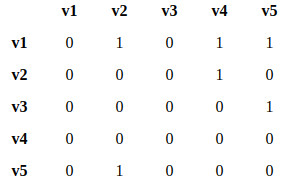
\includegraphics[height=3cm]{./img/lecture3-fig6b.jpg}
 \end{center}
%http://ceadserv1.nku.edu/longa//classes/mat385_resources/docs/matrix.html

{\bf Question.}  What is the sum of the entries in a row of the adjacency
matrix for a directed graph?
 \vspace{.5in}
    
\end{frame}

\end{document}
